\documentclass[a4paper,12pt]{article}

\usepackage[utf8x]{inputenc}
\usepackage[english,ngerman]{babel}
\selectlanguage{ngerman}

\usepackage[T1]{fontenc}
\usepackage{amsmath}
\usepackage{graphicx}
\usepackage{graphviz}

\usepackage{amsfonts}

\usepackage{url}
\usepackage[colorlinks=false,pdfborder={0 0 0},breaklinks=true]{hyperref}

\usepackage[toc,nopostdot,nonumberlist,acronym]{glossaries}
\newglossaryentry{gls-rpi}
{
  name={RaspBerry Pi},
  description={Kleiner Einplatinencomputer im Kreditkartenformat, entwickelt von
    der \emph{Raspberry Pi Foundation}.	Basiert auf einem ein Ein-Chip-System von Broadcom
    mit einem ARM-Mikroprozessor und kostet zwischen 25 und 35\$.},
}
\newglossaryentry{gls-zb}
{
  name={ZigBee},
  description={Spezifikation für drahtlose Netzwerke mit geringem Datenaufkommen,
    wie z. B. Hausautomation, Sensornetzwerke, Lichttechnik. Der Schwerpunkt von
    ZigBee liegt in kurzreichweitigen Netzwerken (10 bis 100 Meter).
    \newline \url{http://www.zigbee.org}}
}
\newglossaryentry{gls-gatt}
{
  name={Generic Attribute Profile},
  description={\gls{gls-bt-profil} zur ernergieeffizienten Übertragung von Sensordaten und kleiner
    Datenmengen.},
}
\newglossaryentry{gls-bt-profil}
{
  name={Bluetooth-Profil},
  description={Schnittstellenspezifikation der Bluetooth Special Interest Group für die drahtlose
    Kommunikation in einer Bluetooth-Umgebung.},
}
\newglossaryentry{gls-apt}
{
  name={Advanced Packaging Tool},
  description={Paketverwaltungssystem aus dem Bereich von Debian/Ubuntu mit dem Ziel
    eine einfache Möglichkeit zur Suche, Installation und Aktualisierung von Programmpaketen
    zur Verfügung zu stellen.},
}
\newglossaryentry{gls-rb}
{
  name={Ruby},
  description={Einfach zu lesende, objektorierte, höhere Programmiersprache deren Programme
    zur Laufzeit interpretiert werden.},
}

\newacronym{apt}{APT}{\gls{gls-apt}}
\newacronym{rpi}{RPi}{\gls{gls-rpi}}
\newacronym{gatt}{GATT}{\gls{gls-gatt}}
\newacronym{gpio}{GPIO}{General Purpose Input/Output}
\newacronym{uart}{UART}{Universal Asynchronous Receiver Transmitter}
\newacronym{deconz}{deCONZ}{dresden elektronik CONtrol Zigbee
  \newline \url{https://www.dresden-elektronik.de/funktechnik/products/software/pc/deconz/}}
\newacronym{noobs}{NOOBS}{New Out Of the Box Software}
\makeglossaries

\usepackage{setspace}

\usepackage{listings}
\usepackage{color}
 
\definecolor{codegreen}{rgb}{0,0.2,0}
\definecolor{codegray}{rgb}{0.95,0.95,0.95}
\definecolor{codepurple}{rgb}{0.58,0,0.82}
\definecolor{backcolour}{rgb}{0.95,0.95,0.92}
 
\lstdefinestyle{mystyle}{
  backgroundcolor=\color{codegray},   
  commentstyle=\color{codegreen},
  keywordstyle=\color{magenta},
  numberstyle=\tiny\color{black},
  stringstyle=\color{codepurple},
  breakatwhitespace=false,         
  breaklines=true,                 
  captionpos=b,                    
  keepspaces=true,                 
  numbers=left,                    
  numbersep=5pt,                  
  showspaces=false,                
  showstringspaces=false,
  showtabs=false,                  
  tabsize=2
}
\lstset{style=mystyle,basicstyle=\ttfamily,escapeinside=||}

\begin{document}

\title{DAT-Projekt Lichtsteuerung}
\author{Marius \textbf{Schuller}\\
        Stefan \textbf{Thiemann}\\
		Patrick \textbf{Wildt}}
\maketitle

\newpage

\tableofcontents

\onehalfspacing

\newpage

\section{Einführung}
\label{einfuehrung}

Im Zuge der Internet-of-Things-Kampagne\footnote{\url{http://www.nextgenerationmedia.de}}
werden immer mehr ``dumme'' bzw. einfache Geräte miteinander vernetzt und die
resultierenden Daten intelligent miteinander verknüpft. Dazu gehören auch Lichter und
Glühbirnen. Zur Vernetzung und Steuerung der Lichter existieren bereits mehrere
aktuelle Technologien. Mit Hilfe einer der standardisierten Technologien möchten wir
einen Controller implementieren, der diese Lichter kontrollieren kann.

\section{Lichtsteuerungs-Technologien}
\label{technology}

Üblicherweise möchten Hersteller ein eigenes Produkt-Ökosystem erstellen, aus dem ein
Anwender nicht oder nur schwer entkommen kann. Hierfür werden von den Herstellern
eigene, unfreie Protokolle implementiert. Beispielsweise bietet
\textit{LimitlessLED}\footnote{\url{http://www.limitlessled.com}} Glühbirnen, welche sich
über 2,4 GHz WLAN in das lokale Netzwerk verbinden. Für die eigentliche
Steuerung wurde dazu eine eigene API entwickelt. Eine weitere bekannte Technologie
zur Steuerung von Geräten ist Bluetooth. Hier ist es derzeit möglich
mit Hilfe des \gls{gatt}, ein eigenes Protokoll zu sprechen. Dies wird bei einigen
smarten Glühbirnen verwendet um ein proprietäres Lichtsteuerungsprotokoll zu implementieren.

Die Bluetooth Konkurrenten \textit{Z-Wave}\footnote{\url{http://www.z-wavealliance.org}} sowie
\textit{\gls{gls-zb}} implementieren wieder jeweils eigene Lichtprotokolle. Diese
sind jedoch für jeden Client des Funkstandards nutzbar, sodass die Hersteller kein
eigenes Protokoll implementieren mussten. Der Funkstandard \gls{gls-zb} wird
von den namhaften Herstellern \textit{Philips} und \textit{Osram} verwendet.

Für das Schwerpunktprojekt würden wir uns auf \gls{gls-zb} kompatible Geräte
konzentrieren. Vor allem die Produkte der
\textit{Philips hue}\footnote{\url{http://www.philips.de/e/hue/hue.html}} Reihe.

\section{Komponenten}
\label{components}

Die eigentliche Logik zur Steuerung der Lichter kann auf einem
\emph{\glslink{gls-rpi}{\gls{rpi}}} implementiert werden. Um den Funkstandard \gls{gls-zb}
sprechen zu können wird ein kompatibles Funkmodul benötigt. Hierfür kann das \textit{RaspBee}-Modul
verwendet werden.
Dieses gibt es in zwei Varianten, \textit{Basic} und \textit{Premium}. Während man mit der
Basic-Variante nur mit 5 Knoten sprechen darf, ist dies bei der Premium-Variante
unbegrenzt. Die Lichter würden aus einem \textit{Philips Hue} Starterkit bestehen.

\section{Hardware}
\label{hardware}

\subsection{RaspBee Premium, Raspberry-Pi Einzeln}

\begin{tabular}{p{2cm}p{4.5cm}p{3cm}p{3cm}}
   Menge & Produkt & Einzelpreis & Gesamtpreis\\
   \hline
   3 & \href{http://www.conrad.de/ce/de/product/1316978/Raspberry-Pi-2-Model-B-1-GB-ohne-Betriebssystem}{RaspberryPi 2} & 42 Euro & 126 Euro\\
   3 & \href{http://www.conrad.de/ce/de/product/1369407/Raspberry-Pi-Erweiterungs-Platine-Zigbee-200-Knotenpunkte-Raspberry-Pi}{RaspBee Premium} & 60 Euro & 180 Euro\\
   3 & \href{http://www.conrad.de/ce/de/product/1314141/Philips-Hue-LED-Leuchtmittel-Erweiterung-E27-9-W-RGB}{Philips Hue LED}
        \newline 1 x 9W A60 E27 & 59 Euro & 177 Euro\\
   \hline
   Gesamtpreis & & & \textbf{483 Euro}\\
\end{tabular}

\subsection{RaspBee Premium, Raspberry-Pi Bundle}

\begin{tabular}{p{2cm}p{4.5cm}p{3cm}p{3cm}}
   Menge & Produkt & Einzelpreis & Gesamtpreis\\
   \hline
   3 & \href{http://www.reichelt.de/Einplatinen-Computer/RASP-2-B-ALL-IN/3/index.html?ACTION=3&GROUPID=6666&ARTICLE=152855}{RaspberryPi 2 Bundle} & 70 Euro & 210 Euro\\
   3 & \href{http://www.conrad.de/ce/de/product/1369407/Raspberry-Pi-Erweiterungs-Platine-Zigbee-200-Knotenpunkte-Raspberry-Pi}{RaspBee Premium} & 60 Euro & 180 Euro\\
   3 & \href{http://www.conrad.de/ce/de/product/1314141/Philips-Hue-LED-Leuchtmittel-Erweiterung-E27-9-W-RGB}{Philips Hue LED}
        \newline 1 x 9W A60 E27 & 59 Euro & 177 Euro\\
   \hline
   Gesamtpreis & & & \textbf{567 Euro}\\
\end{tabular}

\subsection{Hinweis}

Unter Umständen sind Bestandteile der Liste schon im Vorrat der Hochschule oder
der Projektteilnehmer. Je nach Beteiligung der Fachhochschule würden wir für einen
Teil der Kosten aufkommen.

\newpage

\section{Grobarchitektur}
\label{architecture}

In Abbildung \ref{fig:architecture} wird der grobe, vorraussichtliche Ablauf der
Kommunikation aller involvierter Komponenten beschrieben.

\begin{figure}[h!]
	\centering
	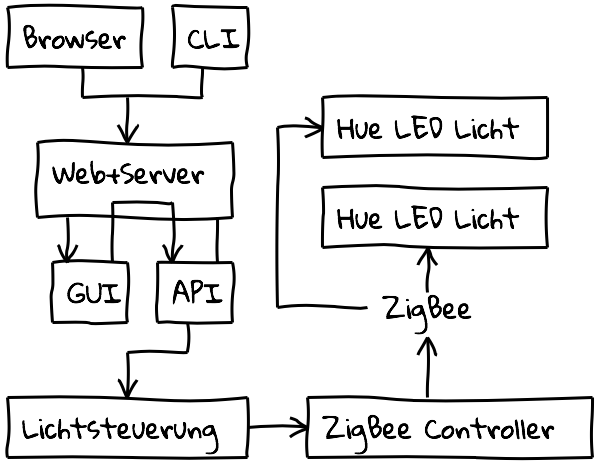
\includegraphics[width=0.9\linewidth]{img/grobarchitektur}
	\caption{Kommunikationsablauf der Komponenten}
	\label{fig:architecture}
\end{figure}

\noindent
Die Lichtsteuerung soll aus mehreren miteinander interagierenden Komponenten
bestehen, die im Folgenden genauer beschrieben werden.

\newpage

\subsection{Hue LED Licht}

Die zu steuernden Lampen werden in eine herkömmliche Fassung geschraubt worüber sie
wie normale Leuchtmittel mit Strom versorgt werden. Die Hue LEDs besitzen dazu aber einen
\gls{gls-zb}-Chip, mit dem sie Teil eines \gls{gls-zb}-Netzwerks werden können. In diesem Netzwerk
fungieren sie als \emph{End Device}, das bedeutet, sie nehmen nicht am Routing innerhalb des
Netzwerks teil, benötigen dafür aber auch nur einen kleinen Teil der Funktionen des
\gls{gls-zb}-Standards. Über das \gls{gls-zb}
\emph{Light Link}-Protokoll\footnote{\url{http://www.zigbee.org/zigbee-for-developers/applicationstandards/zigbee-light-link/}}
können die Lampen angesprochen werden und bestimmte Einstellungen wie Helligkeit und Farbe
eingestellt werden.

\subsection{\gls{gls-zb} Controller}

Der \gls{gls-zb} Controller RaspBee ist die eigentliche Funkeinheit. Sie stellt eine rohe
Programmierschnittstelle bereit, um auf das \gls{gls-zb}-Netzwerk zugreifen zu können.

\begin{figure}[h!]
	\centering
	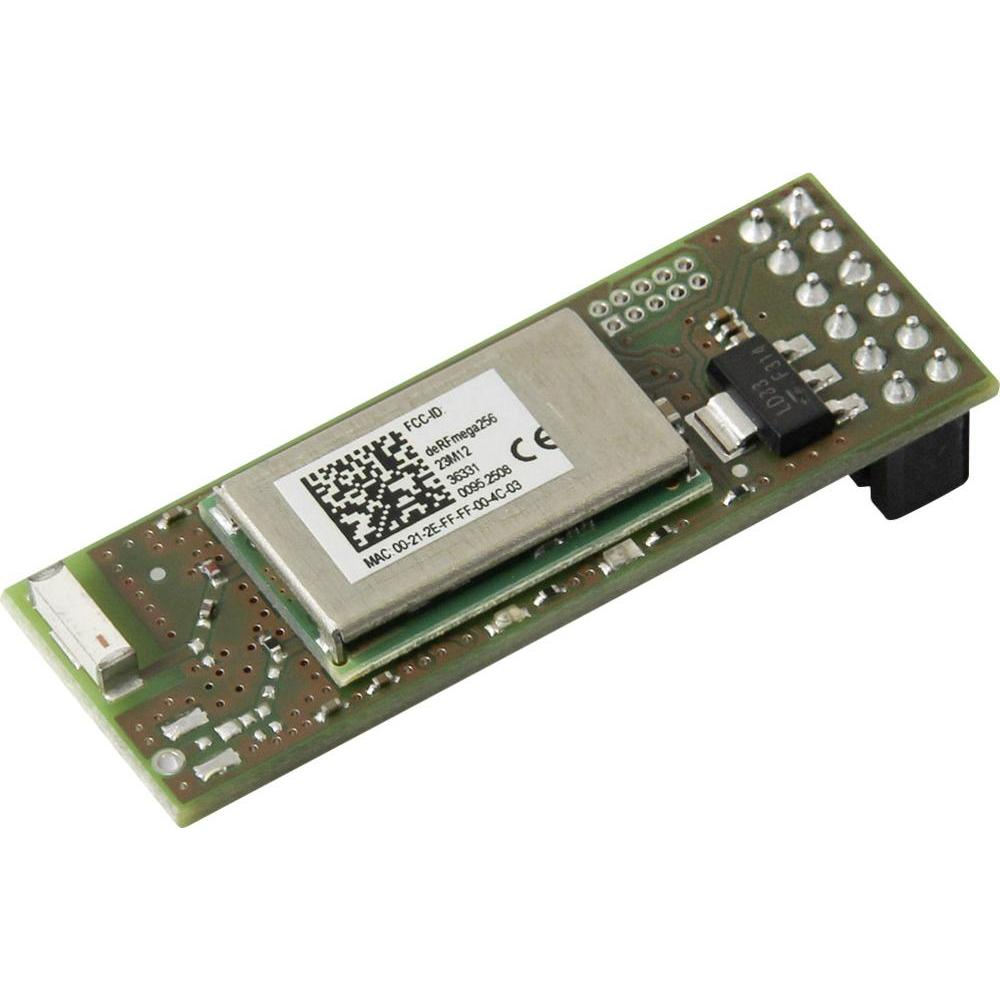
\includegraphics[width=0.4\linewidth]{img/raspbee}
	\caption{RaspBee-Funkmodul}
\end{figure}

\noindent
Der Controller besteht aus zwei Komponenten. Zum einen dem RaspBee, einer
aufsteckbaren Erweiterungsplatine mit Funkmodul für den \gls{rpi}, und zum
anderen dem \gls{rpi} selber. Der \gls{rpi} besitzt eine Reihe an \acrshort{gpio}-Pins am
Rand des Boards.

\begin{figure}[h!]
	\centering
	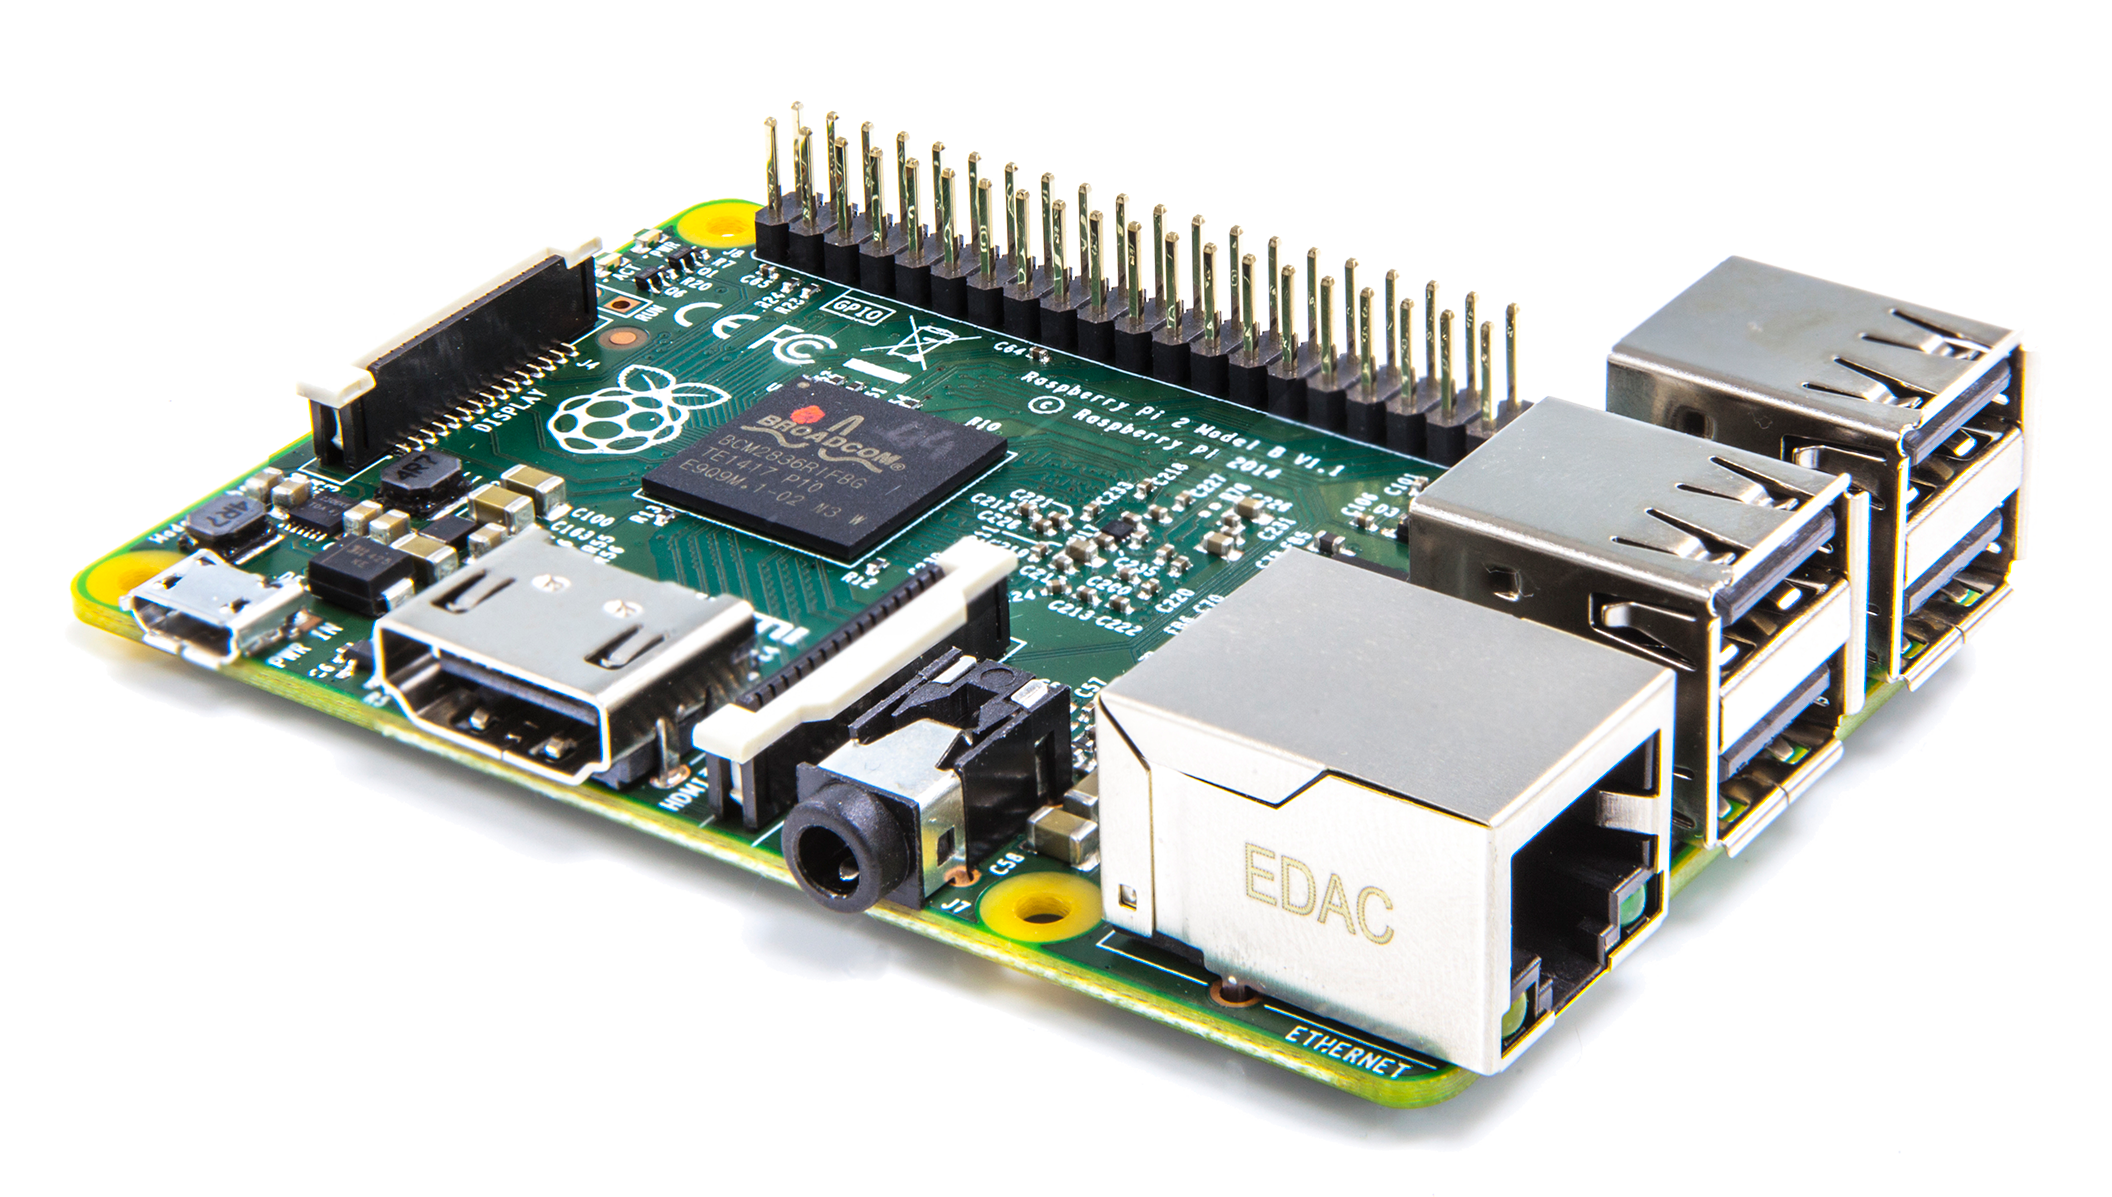
\includegraphics[width=0.7\linewidth]{img/rpi2}
	\caption{Raspberry 2}
\end{figure}

\noindent
Das RaspBee ist an diese \acrshort{gpio}-Pins angepasst und wird dadurch mit Strom versorgt.
Außerdem werden die \acrshort{uart}-Pins zur seriellen Kommunikation mit einem Treiber, der
auf dem \gls{rpi} betrieben wird, verwendet.

\subsection{Lichtsteuerung}

Die Lichtsteuerung soll als hardwarenahes Backend dienen. Diese Software, die auf
dem \gls{rpi} betrieben wird, kommuniziert über die serielle
Schnittstelle mit dem \gls{gls-zb} Controller. Um auf die Nodes des Netzwerks
zugreifen zu können bietet das Backend eine Programmierschnittstelle an.

\subsection{API}

Die API ist eine weitere Software auf dem \gls{rpi}. Sie verwendet
die Schnittstelle der Lichtsteuerung und bietet eine REST-basierte
Webschnittstelle an. Diese Schnittstelle bietet einen vereinfachten Zugriff
auf das Funknetz, mit Fokus auf Steuerung und Verwaltung der Lampen. Durch die
Trennung der einzelnen Programme bleiben Treiber, API und GUI austauschbar.

\subsection{Webserver}

Der Webserver dient primär zum Zugriff auf die Weboberfläche, welche die REST-API
über den Browser zugänglich macht um bequem die Lichter verwalten und steuern
zu können. Weiter wird hier die API etwaigen CLI-Programmen zur Verfügung
gestellt.

\subsection{GUI}

Die GUI, im HTML5 Standard, ist die Schnittstelle zum Benutzer und wird im Browser dargestellt.
Über diese kann der Benutzer die Nodes steuern, wie z.B. Helligkeit und Farbe einstellen.
Zum bequemen Verwenden der API aus dem Browser wird JavaScript auf dem Client verwendet. 

\subsection{CLI}

Um die Lampensteuerung automatisieren zu können, etwa um aus dem Urlaub oder
zeitgesteuert in einem Haus Licht aus- oder anzuschalten, ist ein
Kommandozeileninterface wünschenswert. Für viele Sprachen gibt es bereits
Module mit denen REST-APIs angesprochen werden können, daher ist die
Programmiersprache in der das CLI-Programm umgesetzt werden soll zweitrangig.

\newpage

\section{Umsetzung}
\label{doing}

Umgesetzt und von uns implementiert werden soll die API sowie die CLI. Eine
rudimentäre Umsetzung der Web-GUI ist denkbar, um die prinzipielle Möglichkeit zu
verdeutlichen.
Die Treibersoftware um das RaspBee-Modul anzusteuern ist leider nicht
Open Source. Diese Software bietet eine Programmierschnittstelle, um die eine API
herum entwickelt werden kann.

\subsection{Einschränkungen}

Nach anfänglicher Exploration der mit der RaspBee-Modul zugehörigen Software
von \emph{Dresden Elektronik} wurde festgestellt, dass viel der von uns zu
implementierenden Funktionalität bereits in der bereitgestellten \emph{\acrshort{deconz}}-
Software vorhanden war. Die Anfrage an den Support von Dresden Elektronik
nach Zugang zur Dokumentation der \acrshort{uart}-Schnittstelle und dem Funkmodul
RaspBee wurde verweigert.

Weiter war das Vorhaben aus Punkt \ref{architecture} inhaltlich zu groß gefasst
als dass es in der gegebenen Zeit vollumfänglich durchgeführt werden hätte können.

\section{Installation}

\subsection{Betriebssystem}

Das im \gls{rpi} Bundle aus Punkt \ref{hardware} auf der Micro-SD-Karte vorinstallierte
System heißt \acrshort{noobs} (\acrlong{noobs}).
Dieses System dient als Platform um das eigentliche System zu installieren. Es stellt
eine grafische Oberfläche auf der HDMI-Schnittstelle bereit auf der das über das
Internet zu installierende Betriebssystem ausgewählt werden kann.

Da die \acrshort{deconz}-Software nur in Binärform vorliegt muss ein daran angepasstes
Betriebssystem installiert werden. \emph{Raspbian}\footnote{\url{https://www.raspbian.org/}},
eine für das \gls{rpi} angepasste \emph{Debian}\footnote{\url{https://www.debian.org/}} Version,
ist in der Version Wheezy zur \acrshort{deconz}-Software kompatibel. Weiterhin ist Raspbian eines der 
verbreitetsten Betriebssysteme für den \gls{rpi}.
Wahlweise kann Raspbian auch manuell installiert werden. Dafür muss ein
Image\footnote{\url{https://www.raspberrypi.org/downloads/raspbian/}} der
Version Wheezy heruntergeladen werden. Das Image ist komprimiert und muss nach dem Entpacken auf
die SD-Karte gespielt werden. Das kann mit folgenden Kommandos ausgeführt werden:

\begin{lstlisting}[caption=Raspbian manuell installieren]{RaspbianInstall}
# unzip 2015-05-05-raspbian-wheezy.zip
# dd if=2015-05-05-raspbian-wheezy.img of=/dev/disk
\end{lstlisting}

Der \gls{rpi} bekommt automatisch von einem im Netzwerk verbundenen DHCP-Server
eine IP-Adresse. Diese kann nun entweder über die grafische Oberfläche
abgefragt oder aus dem DHCP-Server ausgelesen werden. Mit Hilfe dieser
Information ist es möglich sich auf den automatisch gestarteten SSH-Server
einzuloggen.

\subsection{\acrshort{deconz}}

Die aktuelle
\acrshort{deconz}-Version\footnote{\url{http://www.dresden-elektronik.de/rpi/deconz/deconz-2.02.05.deb}}
liegt als Debian Paket auf der Website des Herstellers bereit. Nach dem Download
kann die Software mit dpkg installieren. Danach ist die Software betriebsbereit.

\begin{lstlisting}[caption=deCONZ installieren]{deCONZInstall}
# dpkg -i deconz-2.02.05.deb
\end{lstlisting}

\newpage

\section{deCONZ Bedienung}
\label{deconz}

Nachdem man \acrshort{deconz} gestartet hat, werden zwei Bedienoberflächen bereitgestellt.
Eine davon wird als Desktop-Applikation angezeigt. Dort kann sich auf einer hardwarenahen
Ebene verfügbare \gls{gls-zb}-Nodes lassen. Diese Oberfläche kann hauptsächlich zur
Fehlersuche verwendet werden und wird für unseren Zweck nicht direkt benötigt.

Zusätzlich wird auch eine Weboberfläche angeboten, über die die eigentliche Lampen-Steuerung
gemacht werden kann. Es können Gruppen --- Verbünde mehrere Lampen --- und Szenen
--- eigene, gespeicherte Konfigurationen für Lichter und Gruppen --- darüber definiert und
angewählt werden. Im Hintergrund wird eine REST-API bereitgestellt, über die auch dieses
Webinterface die Lichter steuert.

\noindent
Diese API werden wir mit dem hier zu schreibenden Kommandozeilenprogramm verwenden.

\subsection{\acrshort{deconz} starten}

Um deCONZ zu starten muss ein X-Server aktiv sein. \acrshort{deconz} lauscht mit dem
Web-GUI auf Port 80. Optional kann ein anderer Port angegeben werden.

\begin{lstlisting}[caption=deCONZ starten]{deCONZStart}
$ startx &
$ deCONZ --auto-connect=1 --dbg-info=1 &
\end{lstlisting}

\subsection{Web-GUI}
\subsection{API}

\newpage

\section{lolo - Lights on, Lights off}
\label{lolo}

\subsection{Beispielaufrufe}

\begin{lstlisting}[caption=lolo Beispielaufrufe]{loloBeispiel}
$ lolo list

// Gruppe gruppe1 wird erstellt
$ lolo add group gruppe1

// Licht lampe2 wird angelegt und zur gruppe
// 'gruppe1' hinzugef|ü|gt
$ lolo add light lampe2 <UUID> gruppe1

$ lolo lampe1 [on/off]
$ lolo lampe1 red
$ lolo gruppe1 |\#|0412312
$ lolo lampe1 cold
$ lolo gruppe1 warm

// Neue Szene aus aktueller Einstellung von gruppe1,
// lampe3 und lampe4, die nicht in gruppe1 sind
$ lolo add scene szene1 from gruppe1 lampe1 lampe2

// Frauenbesuch aktivieren
$ lolo szene1
\end{lstlisting}

\newpage

\glossarystyle{altlist}
\printglossary[type=\acronymtype,title=Abkürzungsverzeichnis]

\newpage

\printglossary

\end{document}